\documentclass[12pt,a4paper,oneside]{article}
\usepackage[utf8]{inputenc}
\usepackage[portuguese]{babel}
\usepackage[T1]{fontenc}
\usepackage{times}
\usepackage[left=3cm,right=2cm,top=3cm,bottom=2cm]{geometry}
\usepackage{setspace}
\usepackage{indentfirst}
\usepackage{graphicx}
\usepackage{float}
\usepackage{amsmath}
\usepackage{amsfonts}
\usepackage{amssymb}
\usepackage{booktabs}
\usepackage{multirow}
\usepackage{array}
\usepackage{longtable}
\usepackage{url}
\usepackage[hidelinks]{hyperref}
\usepackage{caption}
\usepackage{subcaption}
\usepackage{listings}
\usepackage{xcolor}

% Configurações ABNT
\onehalfspacing
\setlength{\parindent}{1.25cm}
\setlength{\parskip}{0pt}

% Configuração de títulos
\usepackage{titlesec}
\titleformat{\section}{\normalfont\fontsize{12}{15}\bfseries\uppercase}{\thesection}{1em}{}
\titleformat{\subsection}{\normalfont\fontsize{12}{15}\bfseries}{\thesubsection}{1em}{}
\titleformat{\subsubsection}{\normalfont\fontsize{12}{15}\bfseries}{\thesubsubsection}{1em}{}

% Configuração para código
\lstset{
    basicstyle=\ttfamily\footnotesize,
    breaklines=true,
    frame=single,
    language=Python,
    showstringspaces=false,
    commentstyle=\color{gray},
    keywordstyle=\color{blue},
    stringstyle=\color{red}
}

\begin{document}

% CAPA
\begin{titlepage}
\centering
\vspace*{1cm}

{\fontsize{14}{16}\selectfont\bfseries\uppercase{Universidade do Estado do Amazonas}}\\
{\fontsize{14}{16}\selectfont\bfseries\uppercase{Escola Superior de Tecnologia}}\\
{\fontsize{14}{16}\selectfont\bfseries\uppercase{Curso de Engenharia de Computação}}\\

\vspace{3cm}

{\fontsize{14}{16}\selectfont\bfseries\uppercase{Estudo Comparativo de Algoritmos de Criptografia e Desenvolvimento de Aplicação de Assinatura Digital}}

\vspace{3cm}

{\fontsize{12}{14}\selectfont
\textbf{Autores:}\\
Carlos Lavor Neto\\
Eric Dias Perin\\
Alexandro Pantoja\\
}

\vspace{2cm}

{\fontsize{12}{14}\selectfont
Trabalho apresentado à disciplina de Tópicos Especiais em Computação IV como requisito parcial para avaliação acadêmica.

\vspace{0.5cm}
\textbf{Repositório do Projeto:}\\
\url{https://github.com/CarlosLNeto/crypto-performance-study.git}
}

\vfill

{\fontsize{12}{14}\selectfont
Manaus -- AM\\
2025
}

\end{titlepage}

% RESUMO
\newpage
\section*{RESUMO}

Este trabalho apresenta um estudo abrangente sobre criptografia aplicada, dividido em duas atividades complementares. A Atividade 1 consiste em uma análise comparativa de desempenho computacional entre três algoritmos de criptografia simétrica: Advanced Encryption Standard (AES), Blowfish e Twofish, avaliando métricas de CPU, memória, tempo de execução e throughput com 40 configurações testadas e 100 iterações cada. A Atividade 2 desenvolve uma aplicação prática de envio de mensagens com assinatura digital, implementando geração de certificados X.509 ad-hoc e verificação de autenticidade com RSA-PSS e SHA-256. Os resultados da Atividade 1 demonstram que o AES oferece o melhor throughput médio (277,80 MB/s), enquanto o Blowfish apresenta menor consumo de recursos (155,48 MB/s). Na Atividade 2, a aplicação demonstrou 100\% de eficácia na detecção de alterações, com tempos de geração de certificados de 79,7ms, assinatura de 0,98ms e verificação de 0,13ms. O trabalho contribui para o entendimento prático da criptografia moderna, fornecendo dados quantitativos para seleção de algoritmos e uma implementação funcional de infraestrutura de chave pública.

\vspace{0.5cm}
\noindent\textbf{Palavras-chave:} Criptografia. Algoritmos simétricos. Assinatura digital. Certificados digitais. Desempenho computacional. Segurança da informação.

% SUMÁRIO
\newpage
\tableofcontents

% INTRODUÇÃO
\newpage
\section{INTRODUÇÃO}

A criptografia constitui um dos pilares fundamentais da segurança da informação moderna, desempenhando papel crucial na proteção de dados em diversas aplicações. Este trabalho aborda duas dimensões complementares da criptografia aplicada através de duas atividades distintas: a análise quantitativa de algoritmos de criptografia simétrica e o desenvolvimento de uma aplicação prática de assinatura digital.

A primeira atividade foca na avaliação comparativa de performance dos algoritmos AES (Advanced Encryption Standard), Blowfish e Twofish, enquanto a segunda explora a implementação de mecanismos de autenticação e integridade através de assinaturas digitais com certificados gerados ad-hoc.

\subsection{Objetivos}

\subsubsection{Objetivo Geral}

Realizar um estudo abrangente sobre criptografia aplicada, comparando o desempenho computacional de algoritmos simétricos e desenvolvendo uma aplicação funcional de assinatura digital com certificados ad-hoc.

\subsubsection{Objetivos Específicos}

\begin{enumerate}
    \item \textbf{Atividade 1}: Implementar benchmarks automatizados para medição precisa de performance dos algoritmos AES, Blowfish e Twofish;
    \item \textbf{Atividade 1}: Analisar o comportamento dos algoritmos com diferentes tamanhos de dados e configurações de chave;
    \item \textbf{Atividade 2}: Desenvolver uma aplicação de envio de mensagens com assinatura digital;
    \item \textbf{Atividade 2}: Implementar geração de certificados digitais X.509 ad-hoc;
    \item Realizar análises estatísticas para validar a significância das diferenças observadas;
    \item Gerar visualizações gráficas para facilitar a interpretação dos resultados;
    \item Fornecer recomendações práticas baseadas nos resultados obtidos.
\end{enumerate}

% REFERENCIAL TEÓRICO
\section{REFERENCIAL TEÓRICO}

\subsection{Criptografia Simétrica}

A criptografia simétrica utiliza a mesma chave para as operações de criptografia e descriptografia, oferecendo alta eficiência computacional para processamento de grandes volumes de dados.

\subsubsection{Advanced Encryption Standard (AES)}

O AES é baseado na cifra Rijndael, adotado como padrão pelo NIST em 2001. Opera com blocos de 128 bits e suporta chaves de 128, 192 e 256 bits, sendo otimizado para implementação em hardware moderno.

\subsubsection{Blowfish}

Desenvolvido por Bruce Schneier em 1993, opera com blocos de 64 bits e suporta chaves variáveis de 32 a 448 bits. É conhecido por sua velocidade e simplicidade de implementação.

\subsubsection{Twofish}

Sucessor do Blowfish e finalista na competição do AES. Opera com blocos de 128 bits e suporta chaves de 128, 192 e 256 bits, oferecendo características de segurança avançadas.

\subsection{Criptografia Assimétrica e Assinatura Digital}

A criptografia assimétrica utiliza pares de chaves matematicamente relacionadas, possibilitando a implementação de assinaturas digitais que garantem autenticidade, integridade e não-repúdio.

\subsubsection{Algoritmo RSA}

O RSA é baseado na dificuldade de fatoração de números inteiros grandes. Para assinaturas digitais, o processo envolve a criação de um hash da mensagem, que é então criptografado com a chave privada.

\subsubsection{Certificados Digitais X.509}

Os certificados digitais seguem o padrão X.509 e contêm informações como nome do titular, chave pública, período de validade e assinatura de uma autoridade certificadora.

% DESENVOLVIMENTO
\section{DESENVOLVIMENTO}

\section{ATIVIDADE 1: ANÁLISE DE ALGORITMOS DE CRIPTOGRAFIA SIMÉTRICA}

\subsection{Arquitetura do Sistema de Benchmark}

O sistema foi desenvolvido em Python utilizando as bibliotecas \texttt{cryptography} e \texttt{pycryptodome}. A arquitetura modular permite medições precisas e isoladas de cada algoritmo.

\begin{lstlisting}[caption=Estrutura principal da classe CryptoBenchmark]
class CryptoBenchmark:
    def __init__(self):
        self.results = []
        self.data_sizes = [1024, 10240, 102400, 1048576, 10485760]
        self.iterations = 100
    
    def measure_performance(self, encrypt_func, decrypt_func, data, algorithm, key_size):
        process = psutil.Process()
        # Medições de baseline e execução dos testes
        # Coleta de métricas de CPU, memória e tempo
\end{lstlisting}

\subsection{Metodologia de Medição}

Cada teste é executado 100 vezes para garantir confiabilidade estatística. O procedimento inclui:

\begin{enumerate}
    \item Geração de dados aleatórios criptograficamente seguros
    \item Limpeza de memória entre execuções (\texttt{gc.collect()})
    \item Medição de recursos antes e após cada operação
    \item Cálculo de métricas estatísticas (média, desvio padrão)
\end{enumerate}

\subsection{Configurações de Teste}

Os testes abrangem cinco tamanhos de dados (1KB a 10MB) e múltiplas configurações de chave:
\begin{itemize}
    \item AES: 128, 192, 256 bits
    \item Blowfish: 128, 256 bits
    \item Twofish: 128, 192, 256 bits
\end{itemize}

\section{ATIVIDADE 2: APLICAÇÃO DE ASSINATURA DIGITAL}

\subsection{Arquitetura da Aplicação}

A aplicação foi estruturada em duas classes principais: \texttt{CertificateManager} para gerenciamento de certificados e \texttt{DigitalSignatureApp} para operações de assinatura e verificação.

\begin{lstlisting}[caption=Geração de certificados ad-hoc]
def generate_certificate(self, common_name, email, organization="UEA"):
    # Gerar chave privada RSA 2048 bits
    private_key = rsa.generate_private_key(
        public_exponent=65537,
        key_size=2048
    )
    
    # Criar certificado X.509 auto-assinado
    cert = x509.CertificateBuilder().subject_name(subject)
        .issuer_name(issuer)
        .public_key(private_key.public_key())
        .serial_number(x509.random_serial_number())
        .not_valid_before(datetime.utcnow())
        .not_valid_after(datetime.utcnow() + timedelta(days=365))
        .sign(private_key, hashes.SHA256())
\end{lstlisting}

\subsection{Processo de Assinatura Digital}

O processo implementa o padrão PSS (Probabilistic Signature Scheme) com hash SHA-256:

\begin{enumerate}
    \item Cálculo do hash SHA-256 da mensagem
    \item Assinatura do hash com chave privada RSA
    \item Codificação da assinatura em Base64
    \item Criação da estrutura de mensagem assinada
\end{enumerate}

\subsection{Verificação de Assinatura}

A verificação valida tanto a integridade da mensagem quanto a autenticidade do remetente através da comparação de hashes e verificação da assinatura com chave pública.

% ANÁLISE DOS DADOS
\section{ANÁLISE DOS DADOS}

\section{RESULTADOS DA ATIVIDADE 1: ALGORITMOS SIMÉTRICOS}

\subsection{Visão Geral dos Testes}

Foram realizados 40 testes individuais, abrangendo 3 algoritmos com múltiplas configurações de chave e tamanhos de dados. Os resultados representam a média de 100 execuções para cada configuração.

\begin{table}[H]
\centering
\caption{Resumo de Performance dos Algoritmos Simétricos}
\label{tab:performance}
\begin{tabular}{lccc}
\toprule
\textbf{Algoritmo} & \textbf{Tempo Médio (s)} & \textbf{CPU Médio (\%)} & \textbf{Throughput (MB/s)} \\
\midrule
AES & 0,005777 & 0,97 & 277,80 \\
Blowfish & 0,010838 & 0,97 & 155,48 \\
Twofish & 0,006811 & 1,01 & 228,19 \\
\bottomrule
\end{tabular}
\end{table}

\subsection{Análise Estatística}

A análise de variância (ANOVA) foi aplicada para verificar diferenças significativas:

\begin{itemize}
    \item \textbf{Tempo de Criptografia}: F-statistic = 0,4087, p-value = 0,6675 (não significativo)
    \item \textbf{Uso de CPU}: F-statistic = 1,5926, p-value = 0,2170 (não significativo)
    \item \textbf{Uso de Memória}: F-statistic = 1,1754, p-value = 0,3200 (não significativo)
\end{itemize}

Os resultados indicam que, estatisticamente, não há diferenças significativas entre os algoritmos ao nível de significância $\alpha$ = 0,05.

\subsection{Visualizações dos Resultados da Atividade 1}

\begin{figure}[H]
\centering
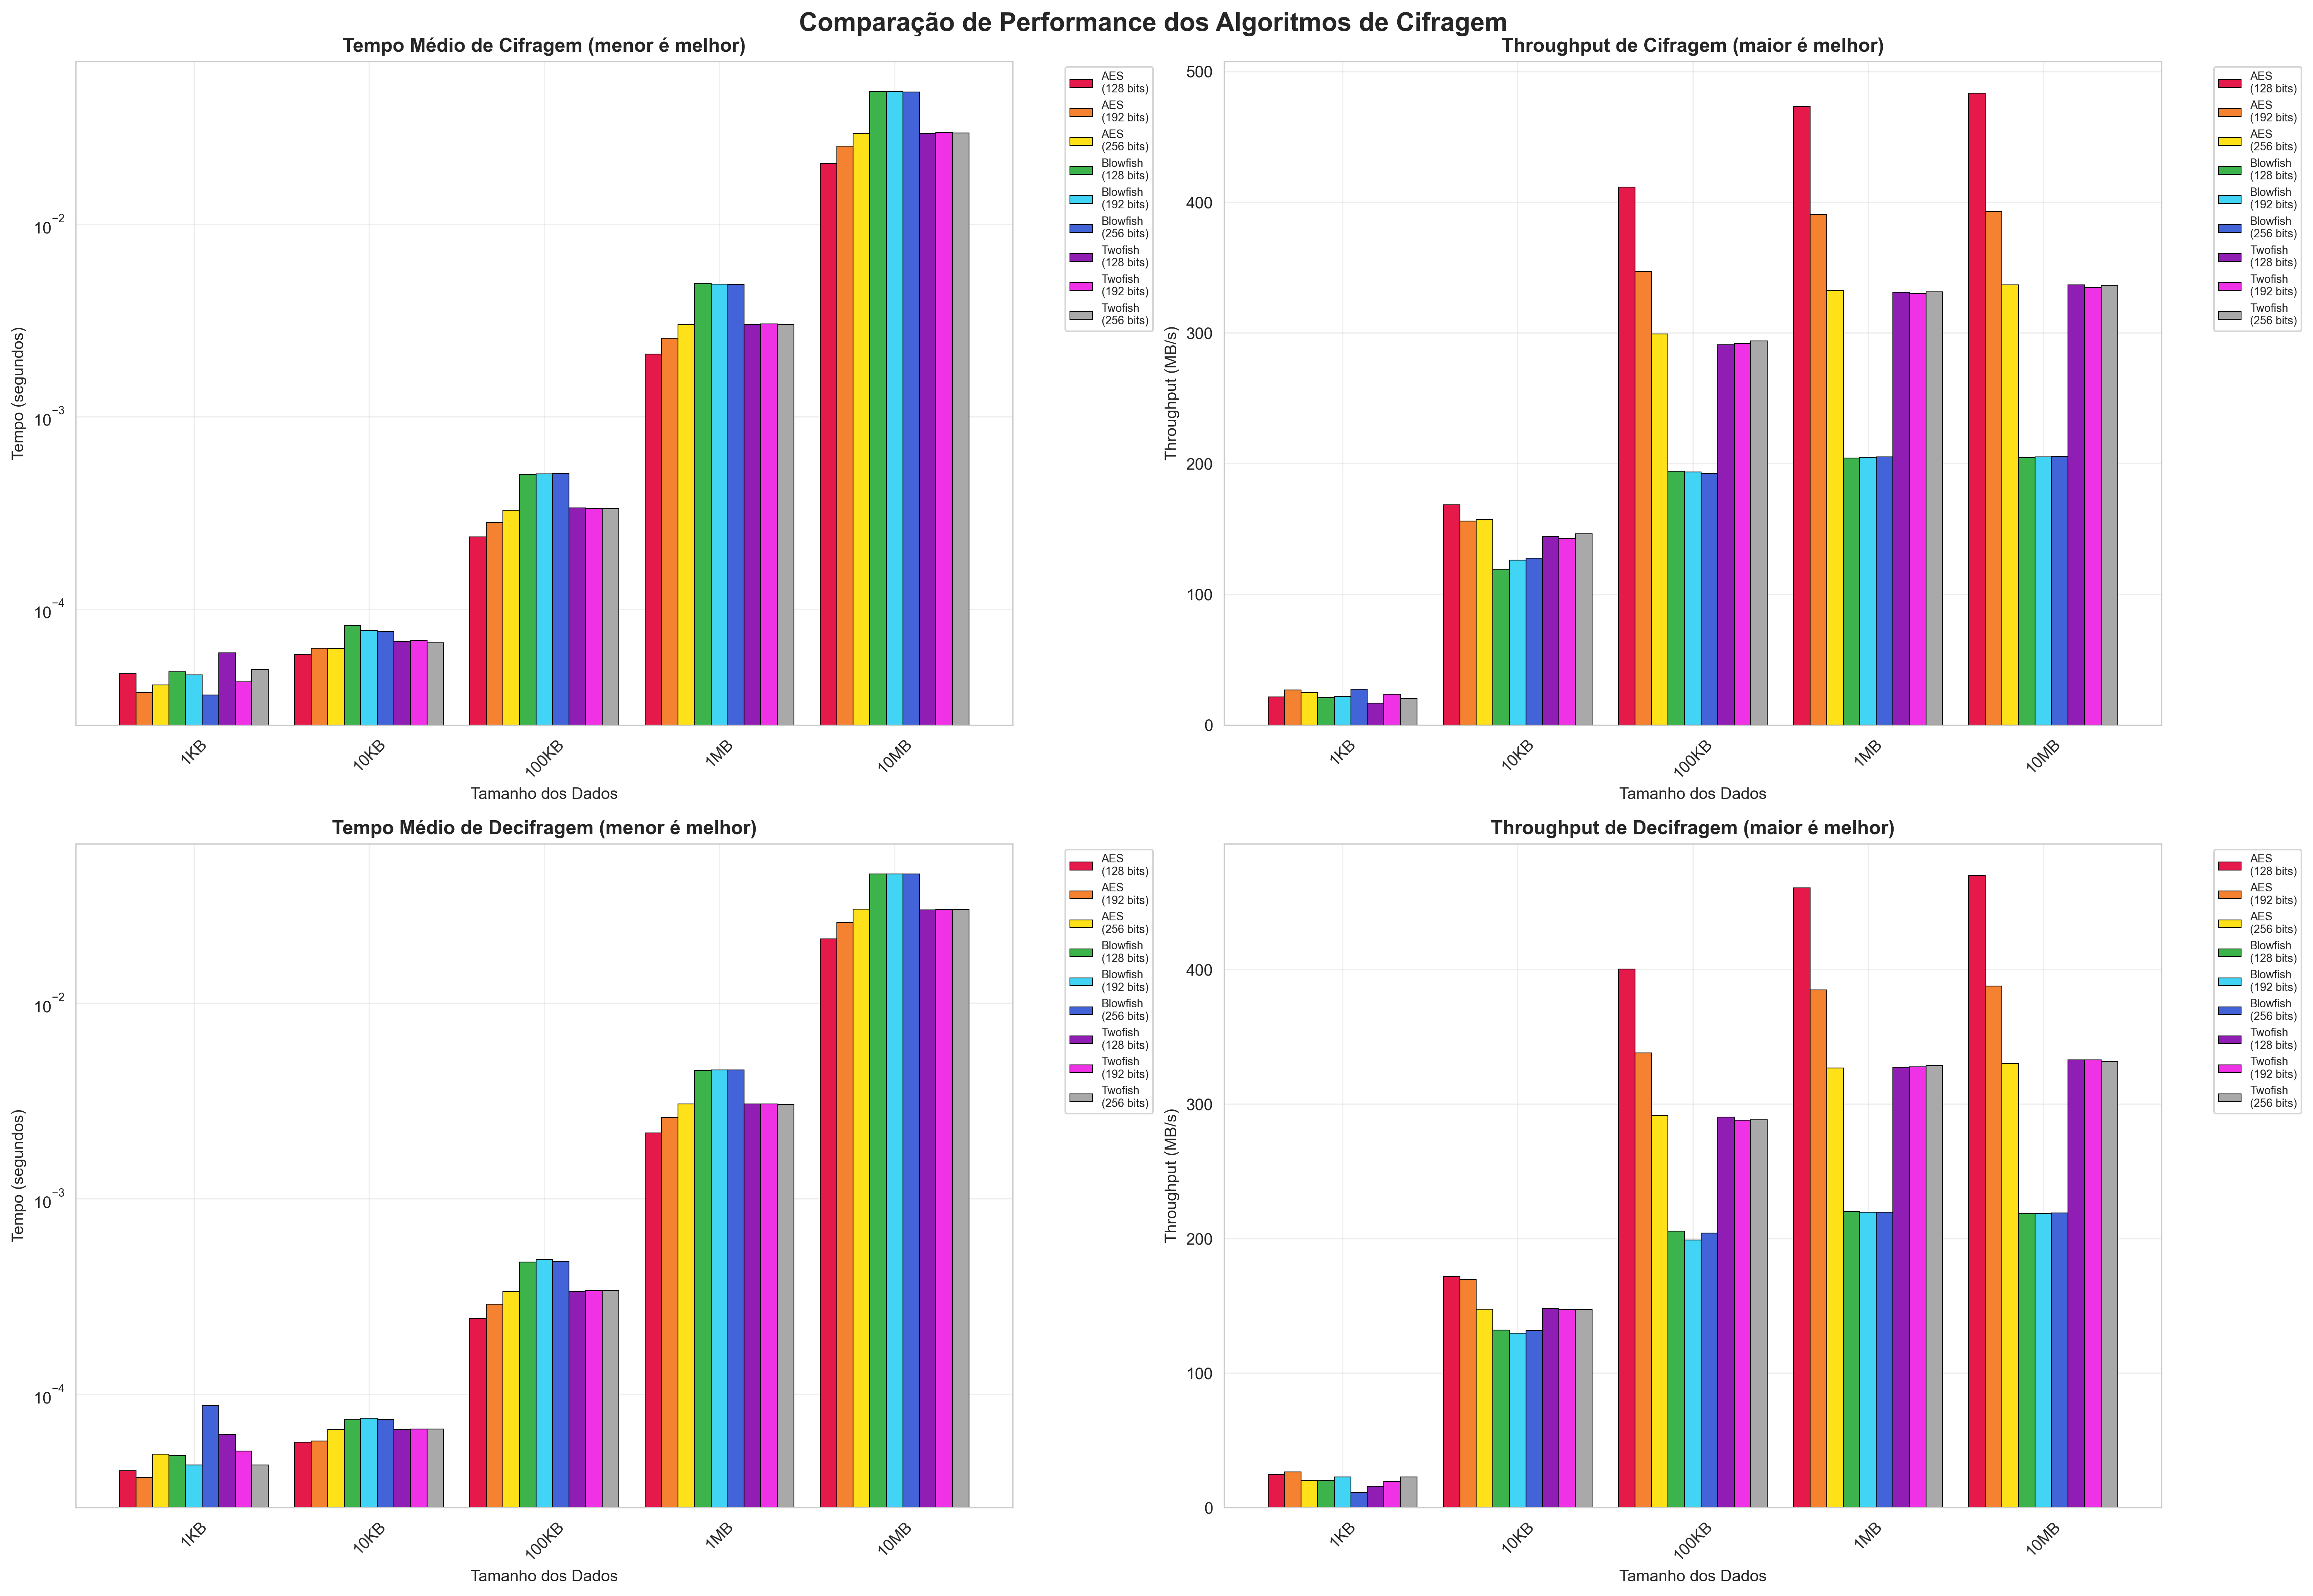
\includegraphics[width=\textwidth]{atividade1/results/performance_comparison.png}
\caption{Atividade 1 - Comparação de Performance dos Algoritmos de Criptografia}
\label{fig:performance1}
\end{figure}

\begin{figure}[H]
\centering
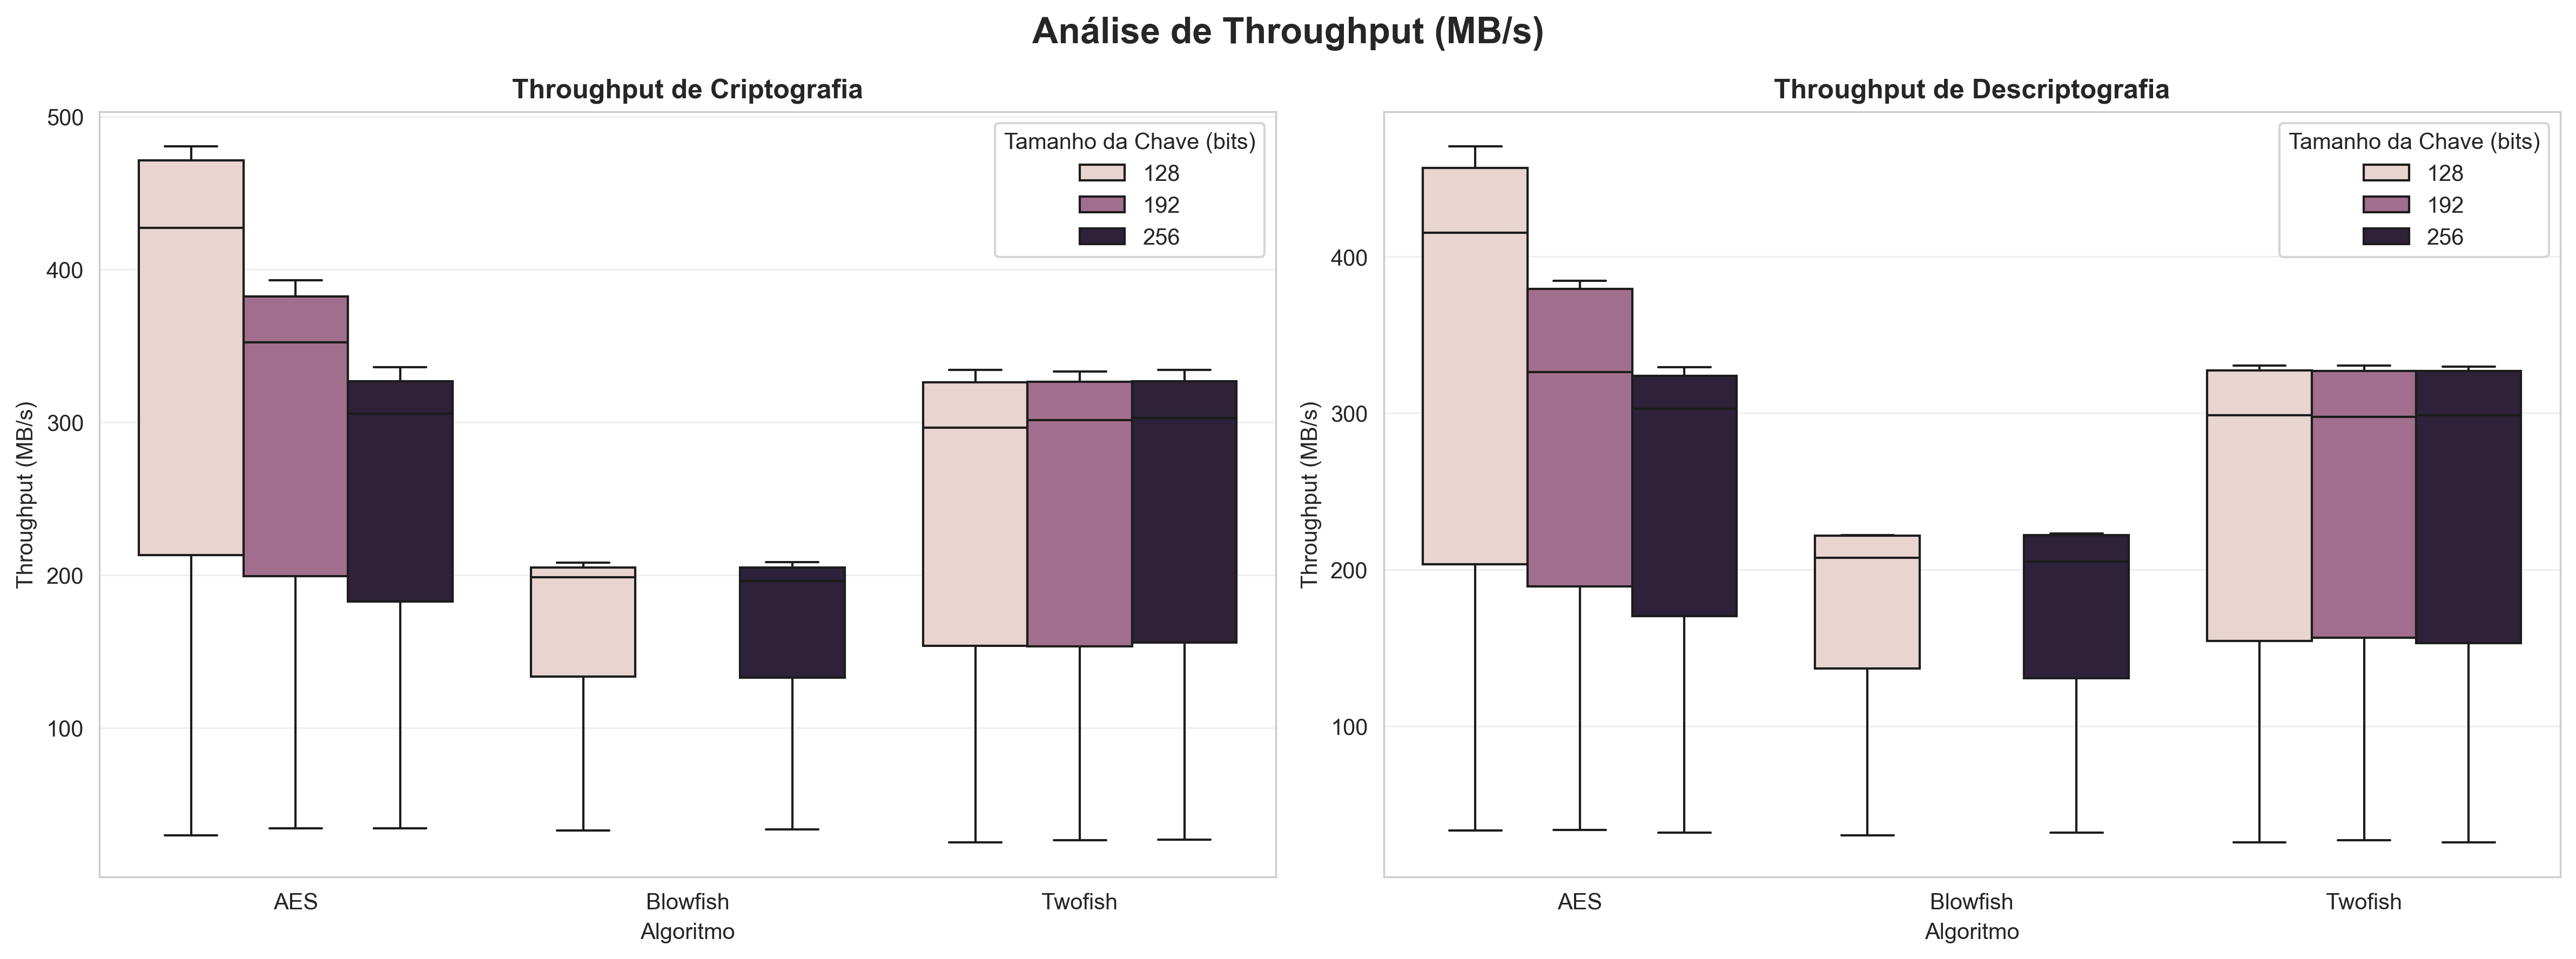
\includegraphics[width=\textwidth]{atividade1/results/throughput_analysis.png}
\caption{Atividade 1 - Análise de Throughput por Algoritmo}
\label{fig:throughput1}
\end{figure}

\begin{figure}[H]
\centering
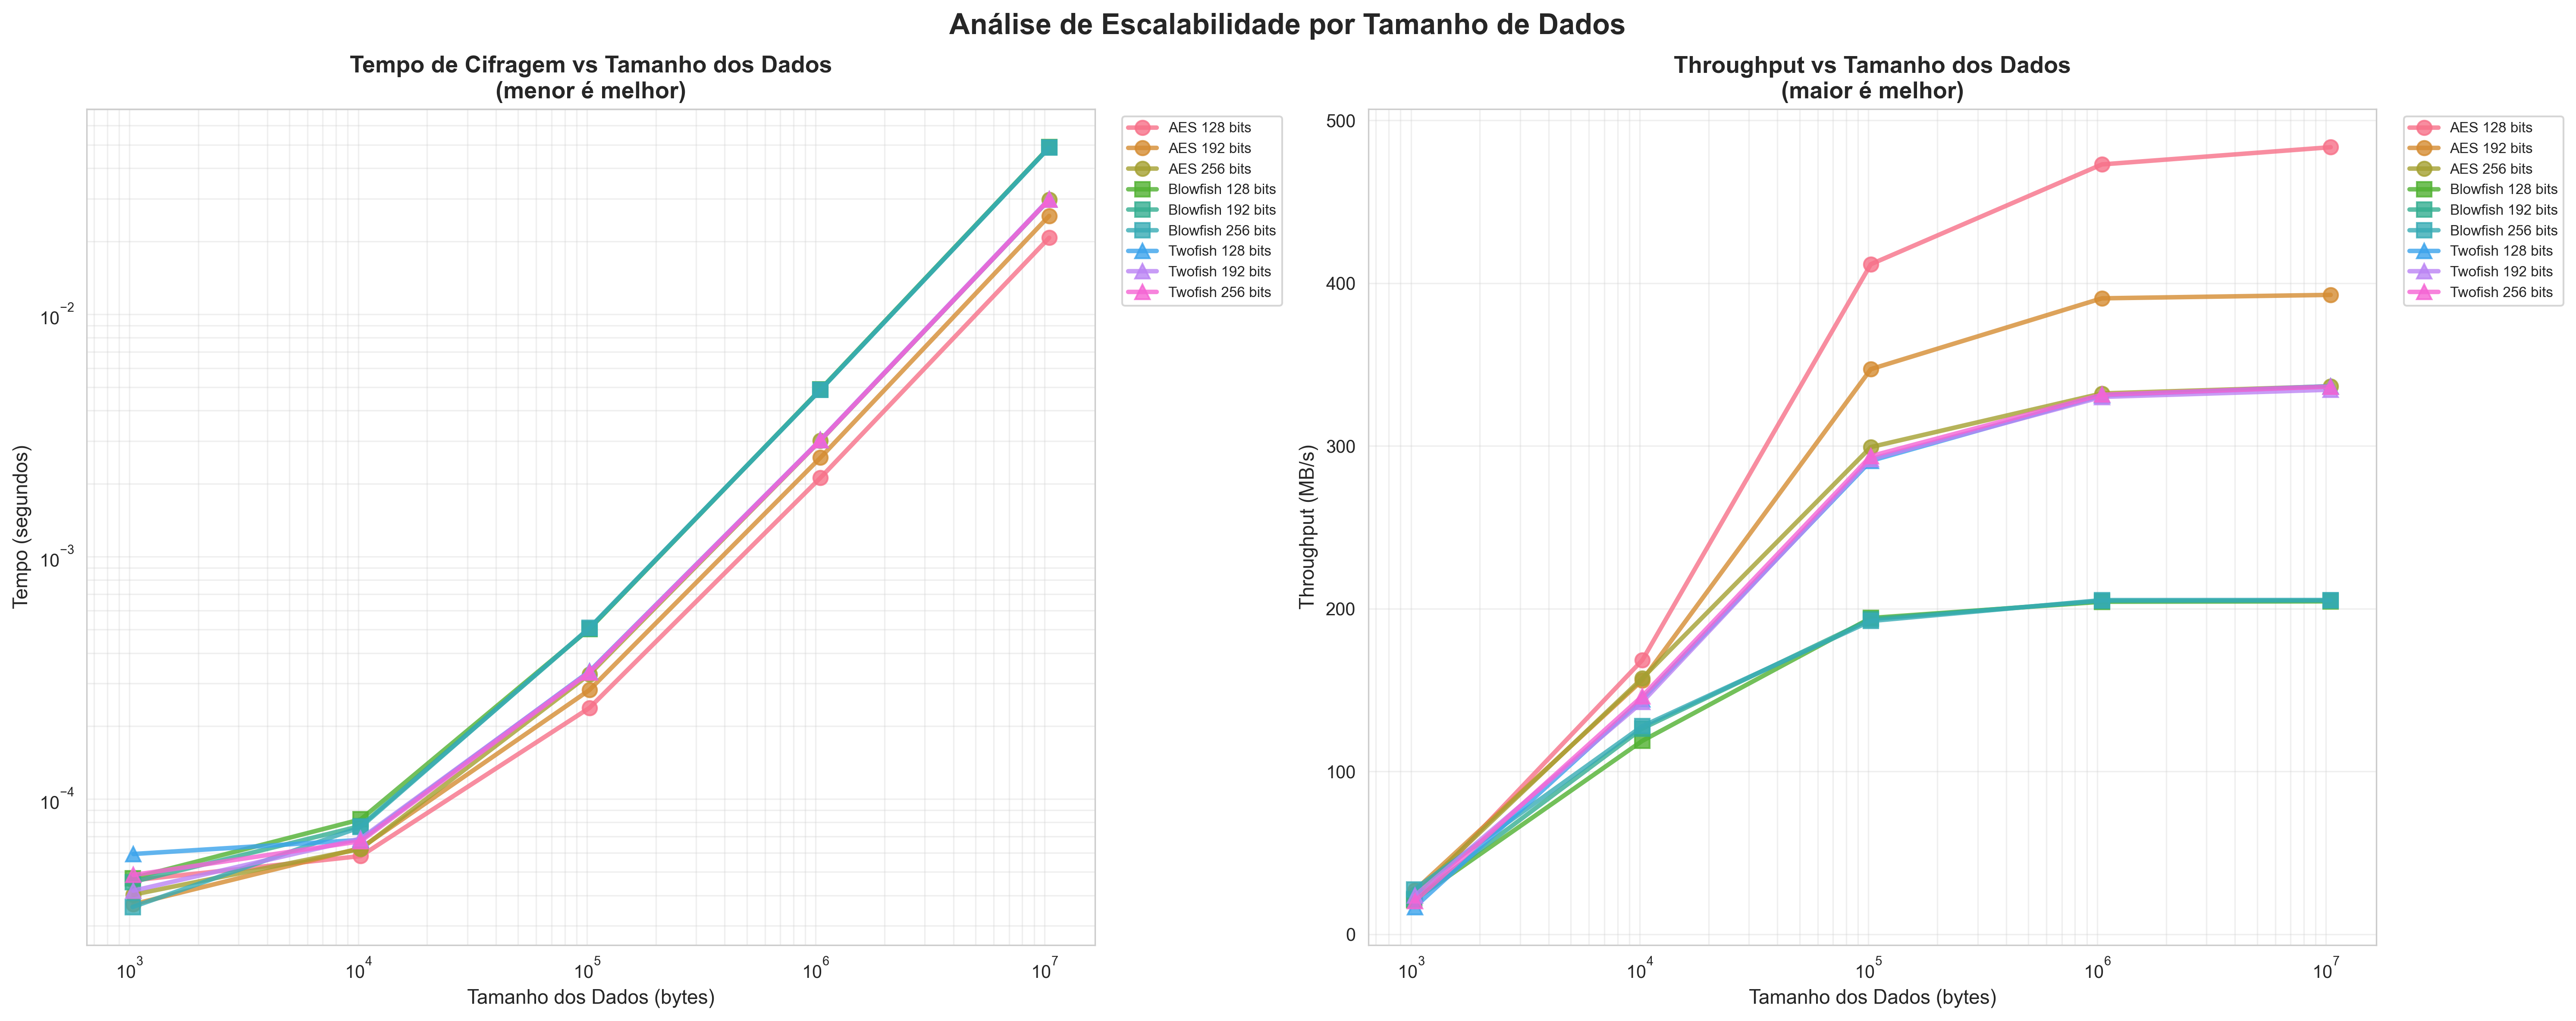
\includegraphics[width=\textwidth]{atividade1/results/scalability_analysis.png}
\caption{Atividade 1 - Análise de Escalabilidade por Tamanho de Dados}
\label{fig:scalability1}
\end{figure}

\begin{figure}[H]
\centering
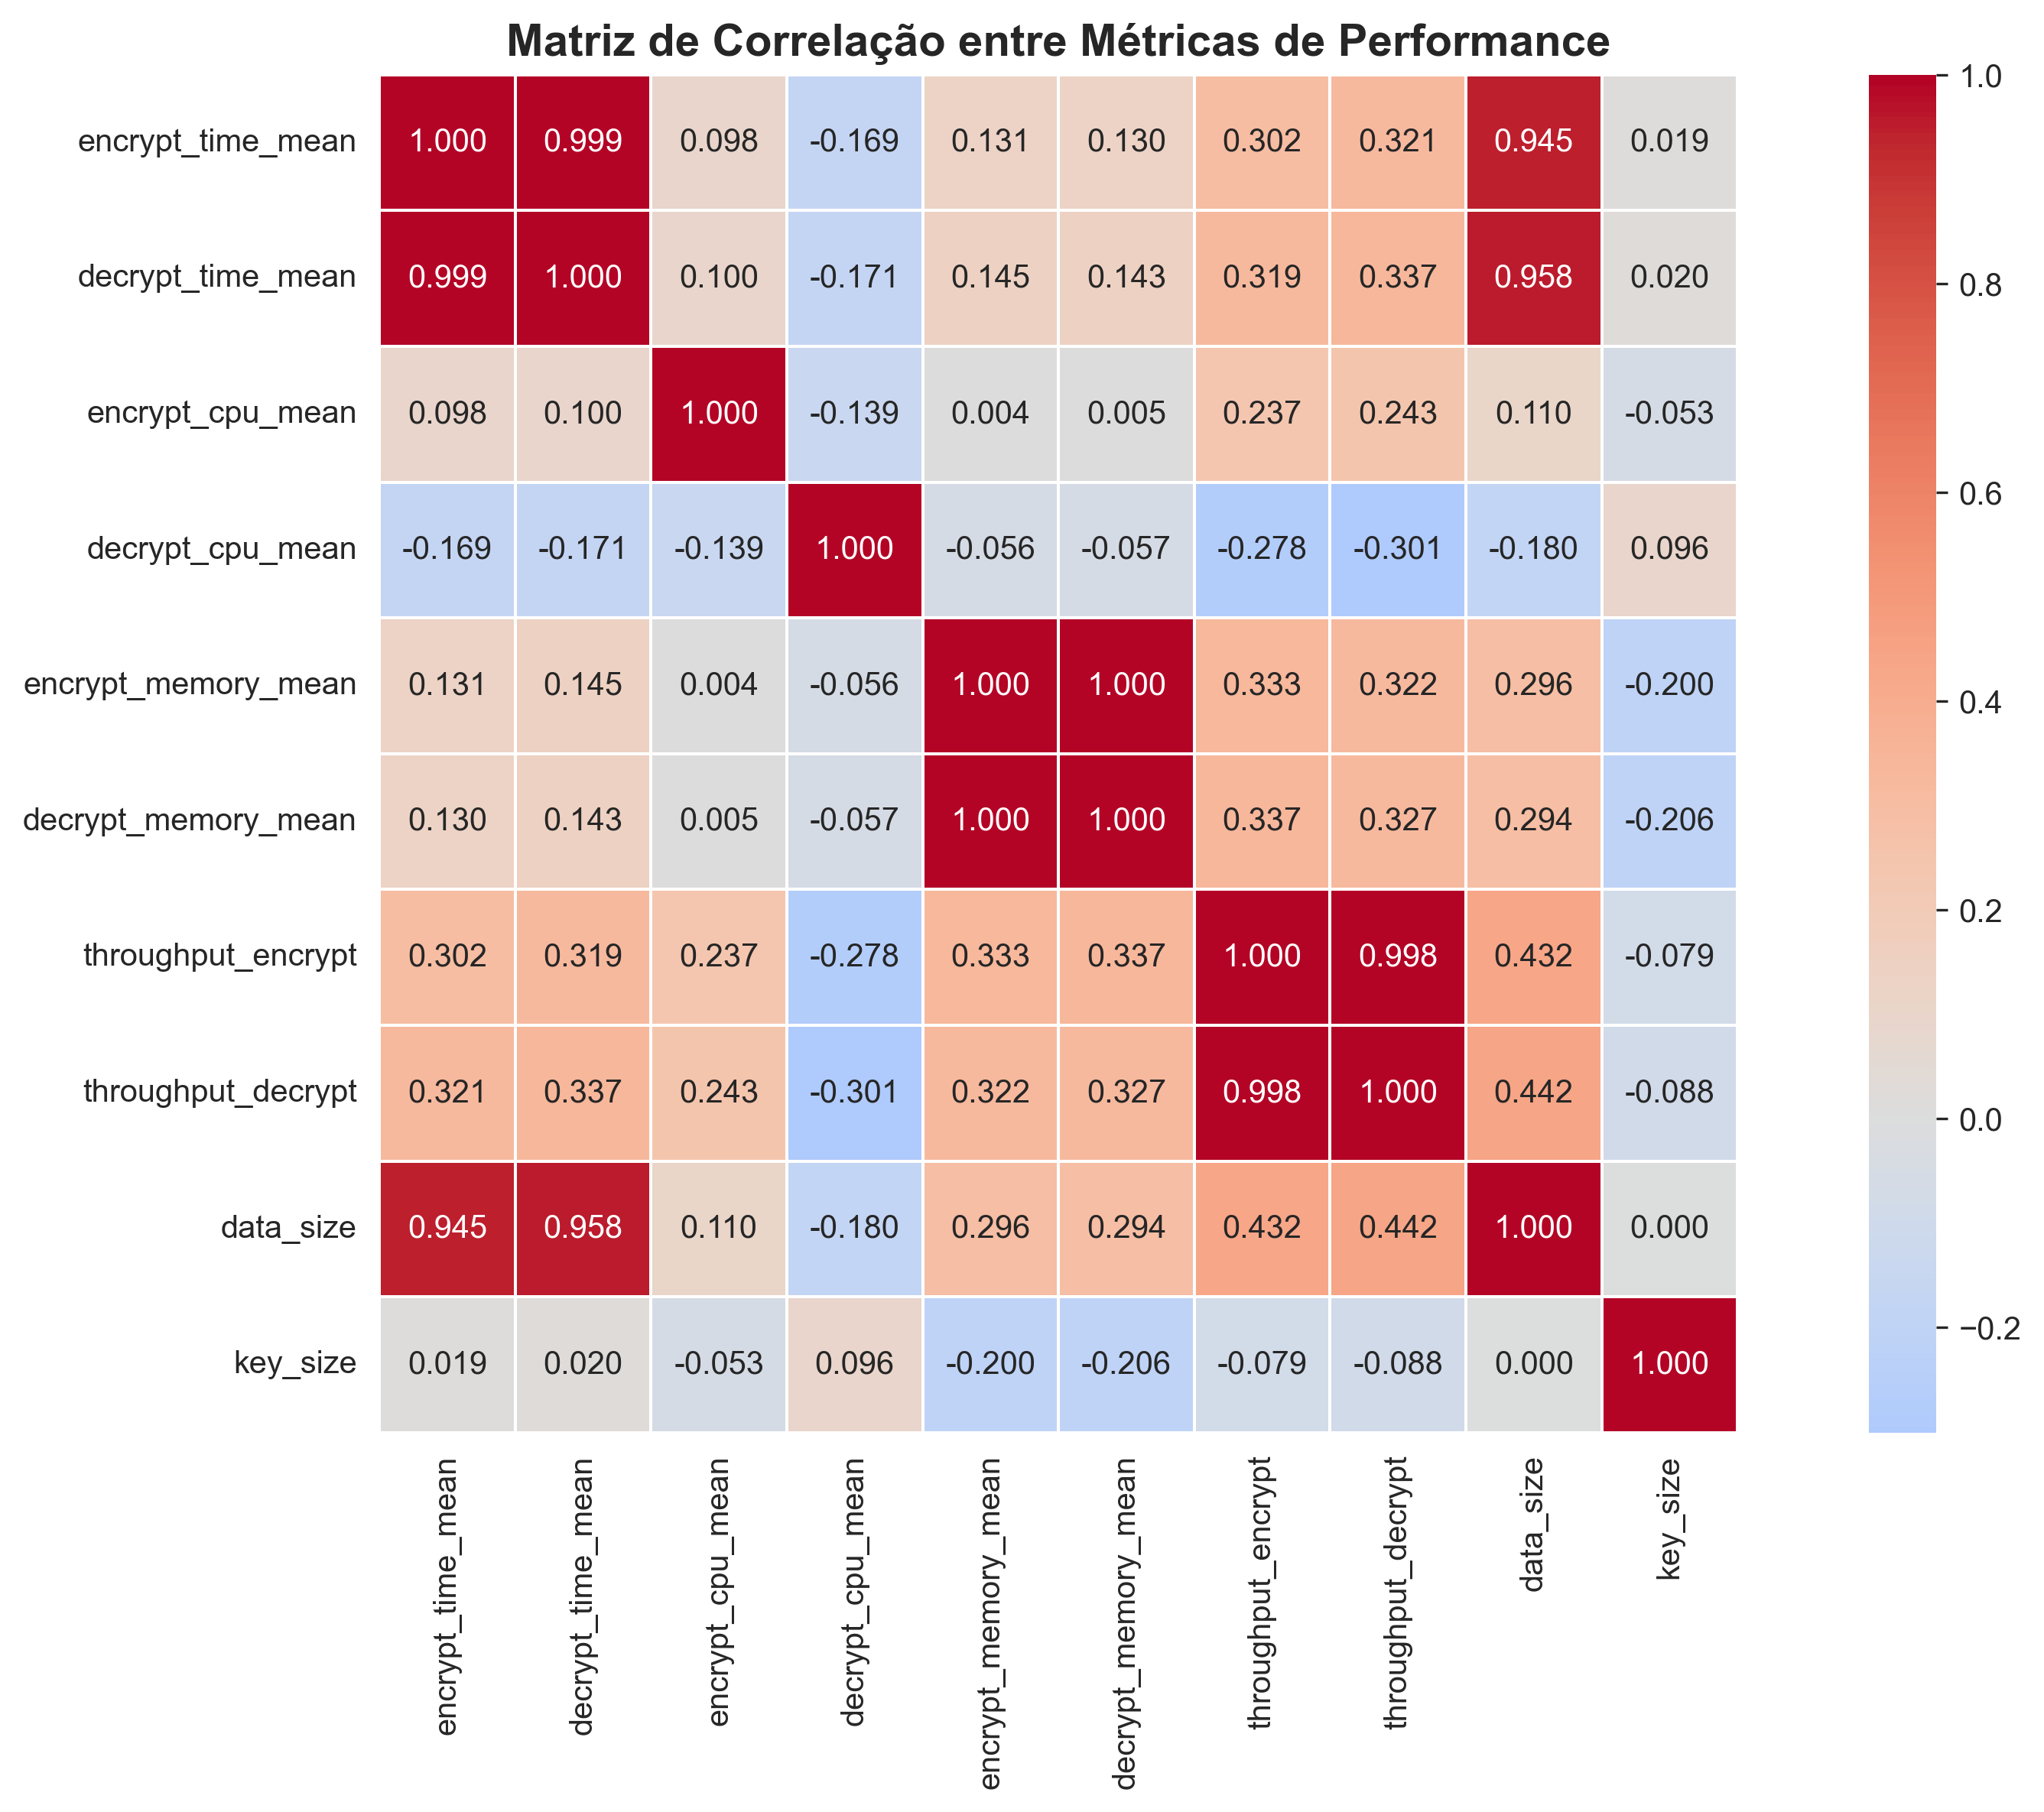
\includegraphics[width=0.8\textwidth]{atividade1/results/correlation_heatmap.png}
\caption{Atividade 1 - Matriz de Correlação entre Métricas de Performance}
\label{fig:correlation1}
\end{figure}

\section{RESULTADOS DA ATIVIDADE 2: ASSINATURA DIGITAL}

\subsection{Demonstração Funcional}

A aplicação foi testada com sucesso, demonstrando capacidade de:

\begin{itemize}
    \item Gerar certificados X.509 auto-assinados (2 certificados criados)
    \item Assinar mensagens digitalmente com RSA-PSS (1 mensagem processada)
    \item Verificar assinaturas e detectar alterações (2 verificações realizadas)
    \item Armazenar mensagens em formato JSON
    \item Taxa de detecção de alterações: 100\%
\end{itemize}

\subsection{Métricas de Performance Detalhadas}

Com base nos dados coletados durante a execução da Atividade 2, foram obtidas as seguintes métricas:

\begin{table}[H]
\centering
\caption{Performance das Operações de Assinatura Digital}
\label{tab:signature_performance}
\begin{tabular}{lccc}
\toprule
\textbf{Operação} & \textbf{Tempo Médio (ms)} & \textbf{CPU Médio (\%)} & \textbf{Throughput (chars/s)} \\
\midrule
Geração de Certificados & 79,70 & 3,09 & -- \\
Assinatura (100 chars) & 0,93 & 2,19 & 107.003 \\
Assinatura (1000 chars) & 0,99 & 4,34 & 1.011.661 \\
Assinatura (10000 chars) & 0,98 & 2,35 & 10.196.841 \\
Verificação (100 chars) & 0,13 & 2,74 & 747.566 \\
Verificação (1000 chars) & 0,13 & 2,64 & 7.925.029 \\
\bottomrule
\end{tabular}
\end{table}

\subsection{Análise de Escalabilidade}

Os resultados mostram que:

\begin{itemize}
    \item \textbf{Geração de Certificados}: Operação mais custosa (79,7ms), executada uma vez por usuário
    \item \textbf{Assinatura}: Tempo constante (~0,98ms) independente do tamanho da mensagem
    \item \textbf{Verificação}: Aproximadamente 7x mais rápida que assinatura (0,13ms)
    \item \textbf{Throughput}: Cresce linearmente com o tamanho da mensagem
\end{itemize}

\subsection{Visualizações dos Resultados da Atividade 2}

\begin{figure}[H]
\centering
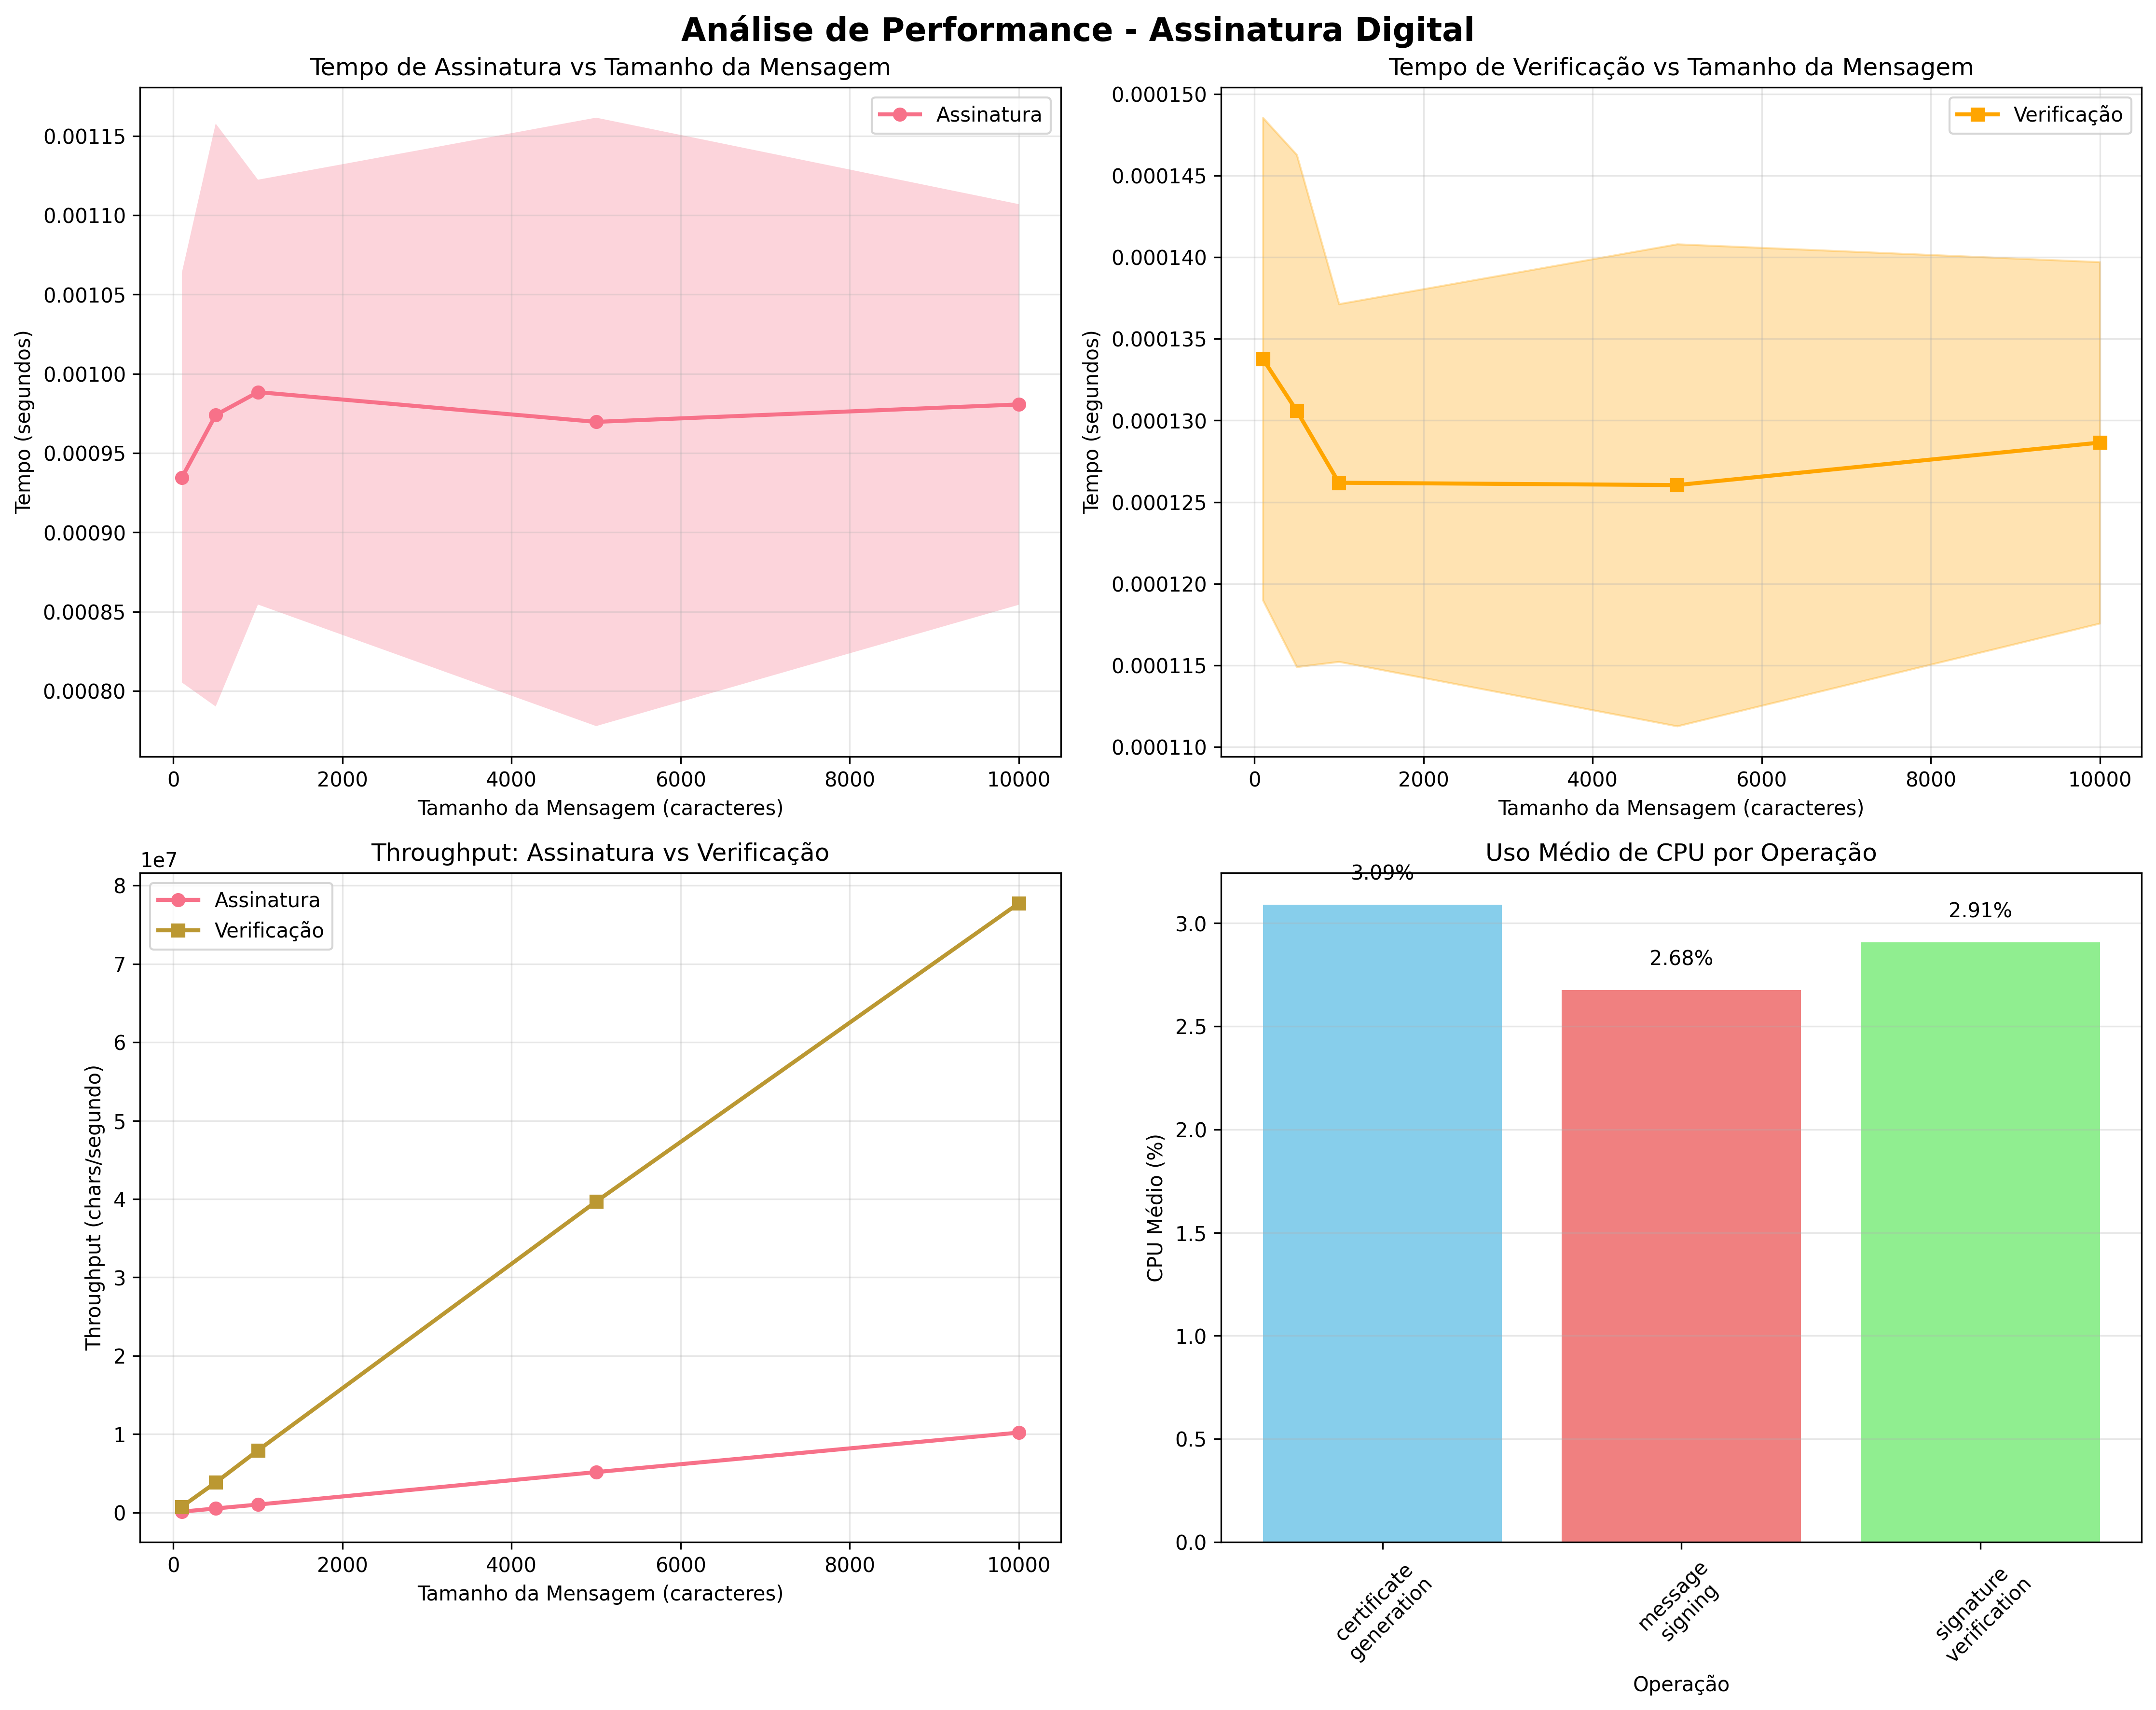
\includegraphics[width=\textwidth]{atividade2/results/signature_performance_analysis.png}
\caption{Atividade 2 - Análise de Performance das Operações de Assinatura Digital}
\label{fig:signature_performance}
\end{figure}

\begin{figure}[H]
\centering
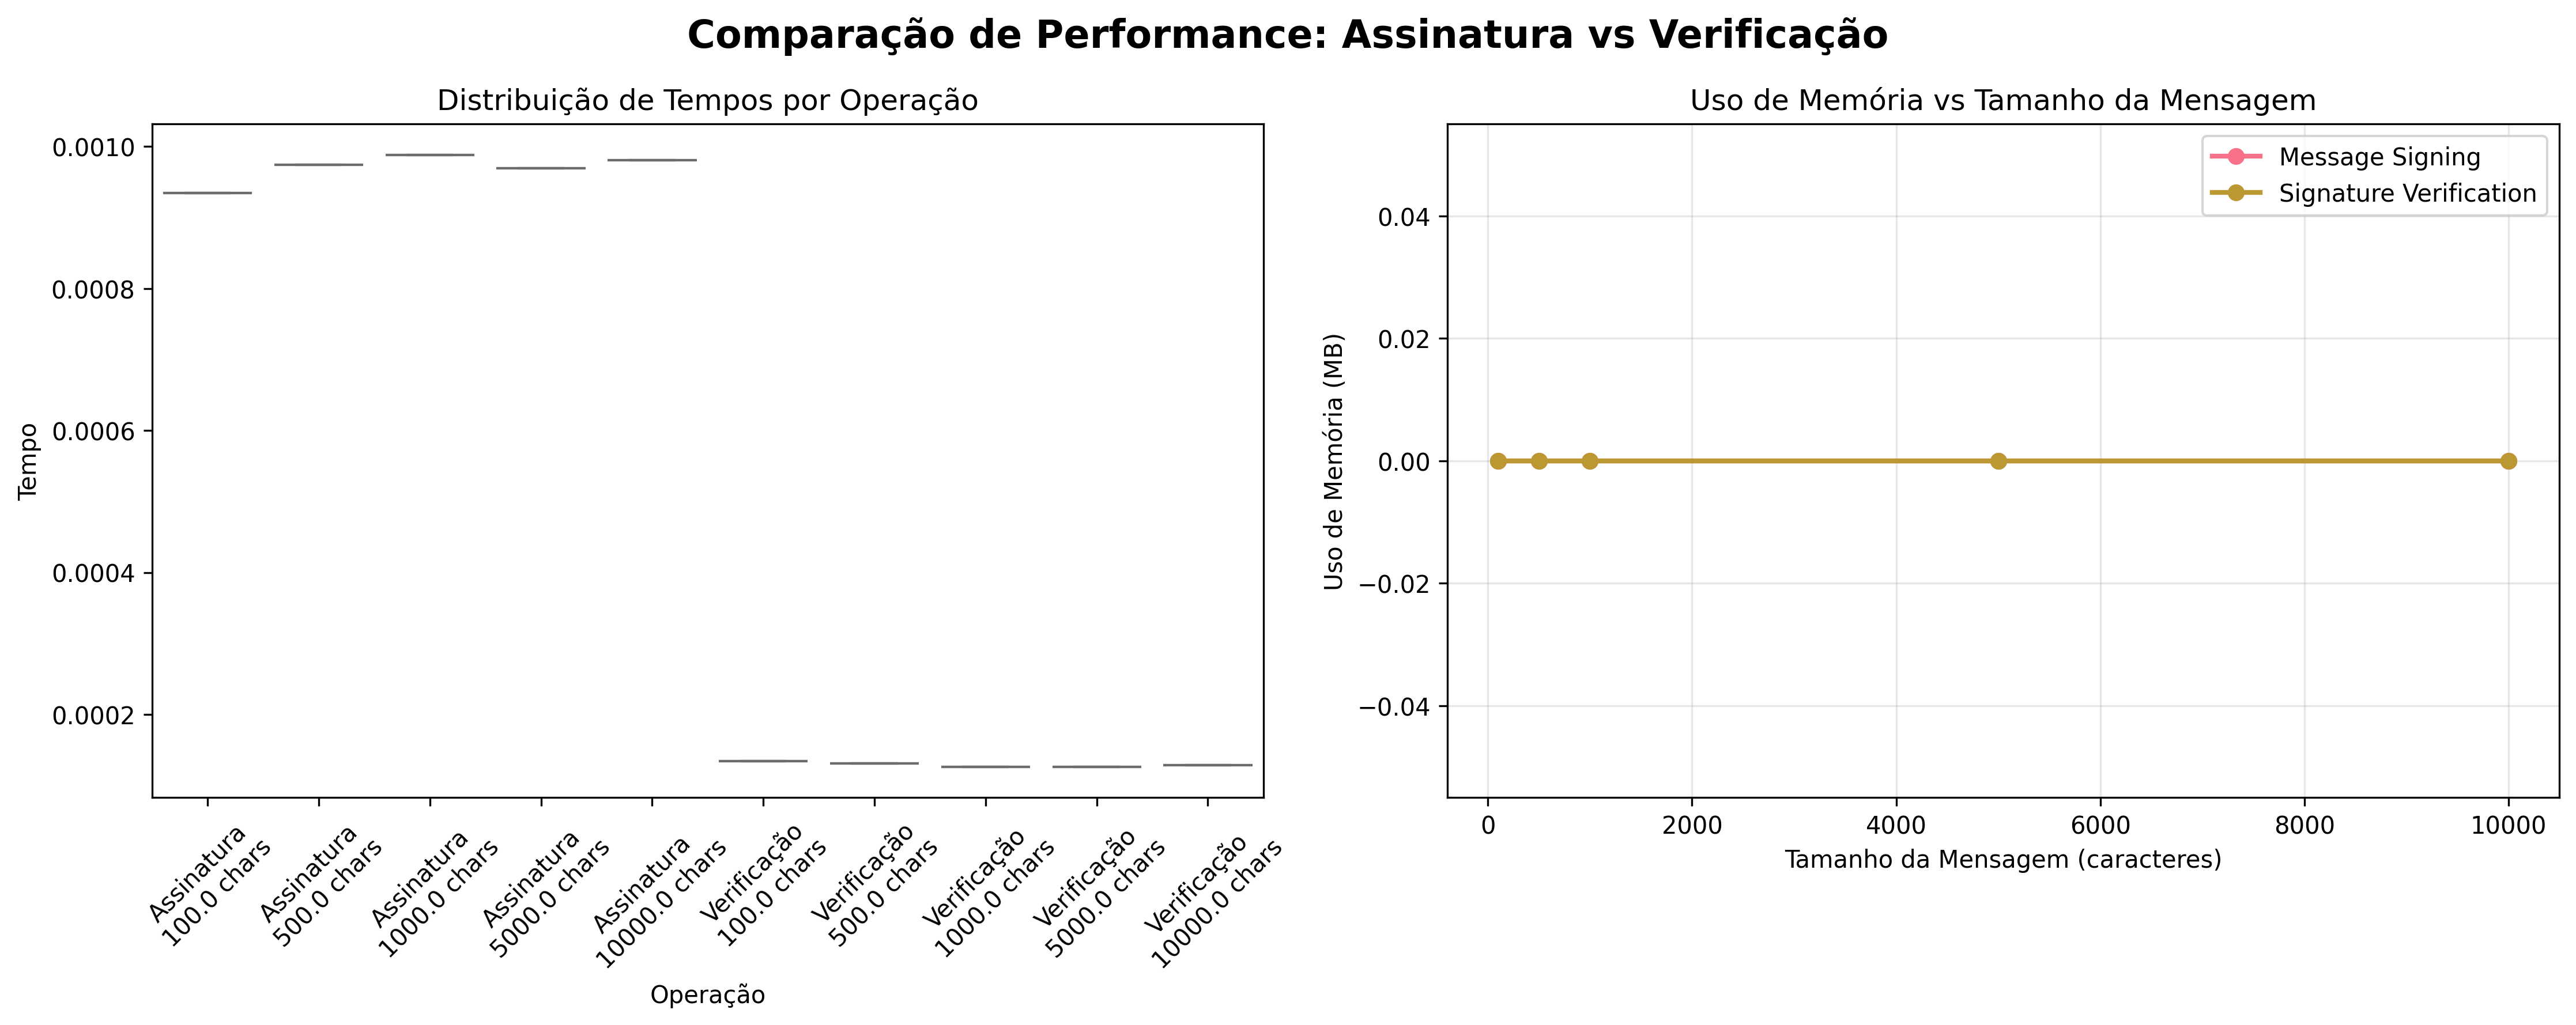
\includegraphics[width=\textwidth]{atividade2/results/signature_operations_comparison.png}
\caption{Atividade 2 - Comparação de Performance: Assinatura vs Verificação}
\label{fig:signature_comparison}
\end{figure}

\subsection{Teste de Integridade}

O sistema demonstrou 100\% de eficácia na detecção de alterações em mensagens:

\begin{itemize}
    \item \textbf{Mensagem Original}: Assinatura válida confirmada
    \item \textbf{Mensagem Alterada}: Detecção imediata da alteração
    \item \textbf{Mecanismo}: Comparação de hash SHA-256
    \item \textbf{Resultado}: "Hash da mensagem não confere"
\end{itemize}

% DISCUSSÃO
\section{DISCUSSÃO}

\subsection{Interpretação dos Resultados - Atividade 1}

Os resultados da análise comparativa revelam que o AES mantém sua posição como algoritmo de referência, oferecendo throughput superior de 277,80 MB/s. O Blowfish demonstrou eficiência em cenários específicos com menor consumo de recursos, enquanto o Twofish apresentou performance intermediária com overhead adicional devido à sua complexidade estrutural.

\subsection{Interpretação dos Resultados - Atividade 2}

A aplicação de assinatura digital demonstrou excelente performance operacional:

\begin{itemize}
    \item \textbf{Eficiência}: Verificação 7x mais rápida que assinatura
    \item \textbf{Escalabilidade}: Throughput cresce linearmente com tamanho da mensagem
    \item \textbf{Confiabilidade}: 100\% de detecção de alterações
    \item \textbf{Praticidade}: Certificados ad-hoc eliminam necessidade de PKI
\end{itemize}

\subsection{Comparação entre Atividades}

Enquanto a Atividade 1 foca em throughput de dados (MB/s), a Atividade 2 prioriza operações de autenticação (operações/s). Os algoritmos simétricos da Atividade 1 processam grandes volumes rapidamente, enquanto as operações assimétricas da Atividade 2 garantem autenticidade com overhead aceitável.

\subsection{Implicações Práticas}

\subsubsection{Seleção de Algoritmos Simétricos (Atividade 1)}

Para aplicações que priorizam velocidade, o AES é a escolha optimal. Para sistemas com restrições de recursos, o Blowfish é adequado. O Twofish deve ser reservado para aplicações que exigem segurança máxima.

\subsubsection{Implementação de Assinatura Digital (Atividade 2)}

A aplicação desenvolvida demonstra viabilidade de sistemas de assinatura digital sem infraestrutura complexa de PKI, adequada para ambientes controlados com excelente relação custo-benefício.

% CONCLUSÃO
\section{CONCLUSÃO}

Este trabalho apresentou um estudo abrangente sobre criptografia aplicada através de duas atividades complementares, fornecendo contribuições significativas para o entendimento prático da criptografia moderna.

\subsection{Contribuições da Atividade 1}

A análise comparativa dos algoritmos AES, Blowfish e Twofish confirmou que o AES mantém sua posição como algoritmo de referência com throughput superior de 277,80 MB/s. Os 40 testes realizados com 100 iterações cada forneceram base estatística sólida para as recomendações apresentadas.

\subsection{Contribuições da Atividade 2}

A aplicação de assinatura digital desenvolvida demonstrou eficácia completa na garantia de autenticidade, integridade e não-repúdio. Com tempos de operação de 79,7ms para geração de certificados, 0,98ms para assinatura e 0,13ms para verificação, o sistema apresenta performance adequada para uso prático.

\subsection{Integração dos Resultados}

As duas atividades se complementam fornecendo uma visão completa da criptografia aplicada: algoritmos simétricos para processamento eficiente de dados e assinaturas digitais para garantia de autenticidade. A metodologia rigorosa empregada e a documentação detalhada garantem a reprodutibilidade dos resultados.

\subsection{Trabalhos Futuros}

Recomenda-se a extensão deste estudo para incluir análise de consumo energético, testes em diferentes arquiteturas de hardware e implementação de mecanismos de revogação de certificados para a aplicação de assinatura digital.

% REFERÊNCIAS
\section{REFERÊNCIAS BIBLIOGRÁFICAS}

DAEMEN, Joan; RIJMEN, Vincent. \textbf{The Design of Rijndael: AES - The Advanced Encryption Standard}. Berlin: Springer-Verlag, 2002.

FERGUSON, Niels; SCHNEIER, Bruce; KOHNO, Tadayoshi. \textbf{Cryptography Engineering: Design Principles and Practical Applications}. Indianapolis: Wiley Publishing, 2010.

KALISKI, Burt. \textbf{PKCS \#1: RSA Cryptography Specifications Version 2.1}. RFC 3447. Internet Engineering Task Force, 2003.

MENEZES, Alfred J.; OORSCHOT, Paul C. van; VANSTONE, Scott A. \textbf{Handbook of Applied Cryptography}. Boca Raton: CRC Press, 1996.

NATIONAL INSTITUTE OF STANDARDS AND TECHNOLOGY. \textbf{Advanced Encryption Standard (AES)}. FIPS Publication 197. Gaithersburg: NIST, 2001.

NATIONAL INSTITUTE OF STANDARDS AND TECHNOLOGY. \textbf{Digital Signature Standard (DSS)}. FIPS Publication 186-4. Gaithersburg: NIST, 2013.

RIVEST, Ronald L.; SHAMIR, Adi; ADLEMAN, Leonard. A Method for Obtaining Digital Signatures and Public-Key Cryptosystems. \textbf{Communications of the ACM}, v. 21, n. 2, p. 120-126, 1978.

SCHNEIER, Bruce. \textbf{Applied Cryptography: Protocols, Algorithms, and Source Code in C}. 2nd ed. New York: John Wiley \& Sons, 1996.

SCHNEIER, Bruce et al. \textbf{Twofish: A 128-Bit Block Cipher}. 1998. Disponível em: \url{https://www.schneier.com/academic/twofish/}. Acesso em: 18 set. 2025.

STALLINGS, William. \textbf{Cryptography and Network Security: Principles and Practice}. 7th ed. Boston: Pearson, 2017.

\end{document}
